%%
%% BioDINO-Edge manuscript formatted for Engineering Applications of Artificial Intelligence (Elsevier)
%% Template: cas-dc (CAS Double Column)
%%
\documentclass[a4paper,fleqn,nologo]{cas-dc}

\usepackage[numbers]{natbib}
\usepackage[protrusion=true,expansion=false]{microtype}
\usepackage{url}
\usepackage{tabularx}
\usepackage{placeins}

%%% Author definitions
\def\tsc#1{\csdef{#1}{\textsc{\lowercase{#1}}\xspace}}
%%%

\begin{document}
\let\WriteBookmarks\relax
\def\floatpagepagefraction{1}
\def\textpagefraction{.001}
\shorttitle{BioDINO-Edge: Gradient-Free Cascades for On-Device Few-Shot Plant Disease Diagnosis}
\shortauthors{R. Javidi Alsaadi and M.R. Samadzadeh}

\title [mode = title]{BioDINO-Edge: Gradient-Free Cascades of Frozen Vision Foundation Models for On-Device Few-Shot Plant Disease Diagnosis}

\author[1]{Reyhane Javidi Alsaadi}
\cormark[1]
\ead{reyhane.code@gmail.com}
\credit{Conceptualization, Methodology, Software, Formal analysis, Investigation, Data curation, Writing - original draft, Visualization}

\author[1]{Mohammad Reza Samadzadeh}
\ead{samadzadeh@ut.ac.ir}
\credit{Conceptualization, Validation, Writing - review \& editing, Supervision, Project administration}

\affiliation[1]{organization={Department of Computer Engineering, Dr. Shariaty Technical University},
                city={Tehran},
                country={Iran}}

\cortext[cor1]{Corresponding author}

\begin{abstract}
Deploying deep neural networks for on-device plant disease diagnosis in precision agriculture is fundamentally constrained by scarce labeled training samples, high-variance vegetative background clutter, and the computational and thermal costs of on-device gradient backpropagation. In this paper, we propose \textbf{BioDINO-Edge}, a gradient-free few-shot diagnostic framework that adapts frozen multi-scale vision foundation models without backpropagation or GPU acceleration. The architecture couples spatial patch representations from DINOv2---capturing fine-grained structural lesion contours and necrotic boundaries---with domain-specialized foliar taxonomic representations from BioCLIP, which fuses visual features with pre-cached Latin botanical prompt ensembles. Under severe few-shot constraints ($K=5$ support leaves per novel class), feature dimensionality exceeds sample size ($N \ll d$), causing empirical within-class covariance matrices to become singular and mathematically non-invertible. We analytically resolve this singularity by regularizing the pooled within-class scatter matrix via closed-form Ledoit--Wolf shrinkage. This regularization provably suppresses shared chlorophyll vegetative background variance by over $31\times$ and enables closed-form Fisher Linear Discriminant Analysis (Fisher-LDA) projection in under 22\,ms on an embedded quad-core CPU. 

During live inference, an adaptive confidence gate combining normalized Shannon predictive entropy and top-2 posterior margin routes routine foliage through an ultra-fast Tier-1 path ($>$45\,FPS, 21.12\,ms latency), while escalating ambiguous field queries to a multimodal Tier-2 classifier. To mitigate empirical prototype drift induced by shifting field illumination and lesion maturity, high-confidence Tier-2 predictions are buffered on-device as reference anchors to periodically recalibrate Tier-2 projection weights via closed-form transductive updates in the background. Packaged into a standalone 22.73\,MB Android APK, BioDINO-Edge achieves 97.37\% $\pm$ 0.73\% 30-episode mean accuracy (peak: 98.72\%, Macro F1: 98.41\%) on the 11-class PlantVillage benchmark with a 0.604\% false-negative escape rate. In cross-domain field evaluation on the in-the-wild PlantDoc benchmark, it attains 83.61\% $\pm$ 11.69\% in 5-way 5-shot episodes and 56.35\% in 27-way all-class simultaneous stress testing, operating entirely offline without requiring remote cloud connectivity.
\end{abstract}

\begin{highlights}
\item Gradient-free foliar pathology adapting frozen DINOv2 and BioCLIP encoders.
\item Analytical Ledoit--Wolf shrinkage resolves small-sample covariance singularity.
\item Joint Shannon-margin confidence gate routes routine leaves to fast 21ms path.
\item Closed-form transductive recalibration adapts to field shifts in under 22ms.
\item Standalone 22.7MB Android APK achieves 97.4\% accuracy without cloud servers.
\end{highlights}

\begin{keywords}
Few-Shot Learning \sep Precision Agriculture \sep Plant Pathology \sep Multimodal Foundation Models \sep Fisher Discriminant Analysis \sep Edge AI \sep Transductive Inference \sep Embedded Computer Vision
\end{keywords}

\maketitle

% =============================================================================
% 1. INTRODUCTION
% =============================================================================
\section{Introduction}
\label{sec:introduction}
Crop pests and foliar diseases destroy an estimated 20\% to 40\% of global agricultural yield annually, incurring over \$220 billion in direct economic losses and severely jeopardizing food security for vulnerable populations \cite{richard2022control}. In conventional agronomic management, disease identification relies heavily on manual scouting and visual inspection by trained phytopathologists \cite{khakimov2022traditional, shoaib2023advanced}. However, manual scouting is labor-intensive, error-prone under field fatigue, geographically unscalable across vast acreages, and susceptible to misdiagnosis when distinct pathogens produce visually homologous symptoms \cite{shoaib2023advanced}.

Deep learning and convolutional architectures have introduced automated alternatives by extracting discriminative lesion representations directly from RGB imagery \cite{shoaib2023advanced}. Nonetheless, conventional supervised paradigms require thousands of curated, expert-annotated images per pathology to train generalized classifiers \cite{shafik2023systematic}. In operational agriculture, such massive datasets are impractical: novel pathogen strains and physiological mutations emerge abruptly with seasonal shifts, while expert botanical labeling remains prohibitively expensive \cite{sun2024few}. Consequently, Few-Shot Learning (FSL) has emerged as an indispensable paradigm: adapting frozen visual backbones to novel disease categories given only a handful ($K=5$) of support leaf samples \cite{snell2017prototypical, sun2024few}.

Recent agricultural FSL literature has explored cross-domain meta-learning architectures such as CDFSL-BDC \cite{yang2024laboratory} and MAFDE-DN4 \cite{zhao2024mafde}, alongside few-shot metric domain adaptation (FMDA) \cite{kudo2025few}, lightweight networks such as AgriFewNet \cite{babu2025agrifewnet}, visual-semantic fusion (VSF) \cite{zhou2026vsf}, and edge-federated frameworks \cite{sharif2026real}. Despite notable progress, four fundamental technical bottlenecks persist in real-world agricultural deployments:
\begin{enumerate}
    \item \textbf{Vegetative Manifold Dominance:} Over 90\% of an infected leaf's visual area comprises healthy green chlorophyll, venation, and natural illumination, while pathological lesions occupy less than 5\%--10\% of the surface \cite{shoaib2023advanced}. In standard feature spaces, isotropic distance metrics (e.g., Euclidean or cosine similarity) are overwhelmed by shared foliar variance, causing severe cross-disease confusion between distinct pathologies of the same host species (e.g., Grape Black Rot vs. Grape Esca) \cite{zhou2026vsf}.
    \item \textbf{High-Dimensional Covariance Singularity ($N \ll d$):} Discriminant metric learning (such as Fisher-LDA) seeks to dampen shared vegetative noise by inverting the within-class covariance matrix \cite{fisher1936use}. However, in scarce 5-shot regimes with high-dimensional foundation embeddings ($d=896$, $N=440$), sample count is substantially smaller than dimensionality, rendering the empirical scatter matrix rank-deficient with hundreds of zero eigenvalues and analytically non-invertible \cite{ledoit2004well}.
    \item \textbf{The Edge Adaptation Paradox:} While parameter-efficient fine-tuning (PEFT) methods such as LoRA \cite{hu2022lora} improve accuracy, on-device backpropagation induces thermal throttling, rapid battery depletion, and high latency on resource-constrained microprocessors (e.g., Raspberry Pi 5, mobile phones, or agricultural scouting drones) \cite{zhao2026lightweight}.
    \item \textbf{Memory \& Rural Connectivity Constraints:} Modern foundation models typically exceed hundreds of megabytes or gigabytes, preventing packaging into lightweight standalone mobile applications suitable for rural areas lacking broadband or cellular connectivity \cite{zhao2026lightweight, sharif2026real}.
\end{enumerate}

To overcome these foundational limitations, we introduce \textbf{BioDINO-Edge}, an entirely gradient-free, two-tier edge framework that couples frozen multi-scale foundation models with analytical closed-form discriminant alignment. DINOv2 Small ($14\times 14$ patches) \cite{oquab2023dinov2} supplies dense patch-level spatial cues for micro-lesion contours, while BioCLIP ViT-B/16 \cite{stevens2024bioclip} provides organismal taxonomic priors. To bypass backpropagation, we formulate an analytical Ledoit--Wolf shrinkage regularizer \cite{ledoit2004well} that guarantees positive-definiteness of the pooled covariance matrix, enabling closed-form Fisher-LDA projection in under 22\,ms. Queries are dynamically routed via a joint margin-entropy Shannon gate \cite{shannon1948mathematical}, achieving over 45\,FPS on routine foliage while escalating ambiguous field leaves to multimodal consensus with background transductive recalibration.

The core scientific and engineering contributions of this work are:
\begin{enumerate}
    \item \textbf{Gradient-Free Dual-Foundation Representation:} We synthesize an 896-dimensional foliar descriptor by coupling self-supervised spatial patch embeddings from DINOv2 with biologically grounded multimodal taxonomic embeddings from BioCLIP, resolving fine foliar necrotic margins without updating backbone parameters.
    \item \textbf{Analytical Covariance Shrinkage \& Fisher Alignment:} We resolve the small-sample singularity problem ($N \ll d$) in few-shot pathology by deriving closed-form Ledoit--Wolf shrinkage on the 896-D joint scatter matrix. This mathematical formulation attenuates shared vegetative background variance by over $31\times$ and computes optimal discriminant boundaries in under 22\,ms on an embedded quad-core CPU.
    \item \textbf{Dual-Process Edge Routing via Shannon Gating:} We implement a cognitive-inspired two-tier architecture where a fast, zero-covariance Tier-1 DINOv2 classifier resolves routine foliage ($>$88\% of queries) at 21.12\,ms ($>$45\,FPS), while an uncertainty gate combining normalized Shannon entropy and top-2 margin escalates ambiguous queries to a multimodal Tier-2 classifier.
    \item \textbf{Soft-Anchored Transductive Recalibration:} To compensate for target-domain centroid shift under field conditions without human labeling, we buffer high-confidence Tier-2 streaming predictions as pseudo-labeled anchors, updating the Tier-2 projection matrix analytically via Cholesky decomposition in the background.
    \item \textbf{Complete Edge Implementation \& Cross-Domain Validation:} We deploy BioDINO-Edge as a fully offline 22.73\,MB Android application. Evaluated over 30 independent Monte Carlo episodes, BioDINO-Edge achieves 97.37\% $\pm$ 0.73\% accuracy (peak: 98.72\%) on 11-class PlantVillage with a 0.604\% false-negative rate, and attains 83.61\% (5-way 5-shot) and 56.35\% (27-way simultaneous) accuracy on the in-the-wild PlantDoc dataset.
\end{enumerate}

% =============================================================================
% 2. METHODOLOGY
% =============================================================================
\section{Methodology}
\label{sec:methodology}

\subsection{Problem Formulation and Mathematical Notation}
\label{sec:notation}
Let $\mathcal{X} \subset \mathbb{R}^{H \times W \times 3}$ denote the space of RGB leaf images. In the few-shot foliar diagnosis setting, we are provided with a novel support set $\mathcal{S} = \{(\mathbf{x}_i, y_i)\}_{i=1}^{N_s}$ containing $K$ labeled support leaf images per novel disease class across $C$ target categories, such that $N_s = C \cdot K$ and $y_i \in \{1, \dots, C\}$. The target novel classes $\mathcal{Y}_{\text{novel}}$ are strictly disjoint from any pretraining base classes ($\mathcal{Y}_{\text{base}} \cap \mathcal{Y}_{\text{novel}} = \emptyset$). Given an unannotated query leaf $\mathbf{x}_q \in \mathcal{Q}$, the diagnostic objective is to predict its disease state $\hat{y}_q \in \{1, \dots, C\}$ with minimal edge latency and zero on-device gradient backpropagation. Table~\ref{tab:notation} outlines the primary mathematical notations employed throughout this paper.

\begin{table*}[htbp]
\centering
\caption{Summary of mathematical notations and descriptions used in BioDINO-Edge.}
\label{tab:notation}
\small
\begin{tabularx}{\textwidth}{lX}
\toprule
\textbf{Notation} & \textbf{Mathematical Description and Operational Meaning} \\
\midrule
$C, K$ & Number of disease classes ($C=11$ in PlantVillage, $C=27$ in PlantDoc) and shots per class ($K=5$). \\
$\phi_{\text{dino}}(\cdot)$ & Frozen DINOv2 Small ($14\times 14$ patches) visual backbone extracting $\mathbf{f}_{\text{dino}} \in \mathbb{R}^{384}$. \\
$\phi_{\text{bio}}(\cdot)$ & Frozen BioCLIP ViT-B/16 visual encoder extracting $\mathbf{f}_{\text{bio}} \in \mathbb{R}^{512}$. \\
$\mathbf{z} \in \mathbb{R}^{896}$ & Concatenated joint foliar descriptor: $\mathbf{z} = [\mathbf{f}_{\text{bio}} \,\|\, \mathbf{f}_{\text{dino}}] \in \mathbb{R}^{896}$. \\
$\mathbf{P}_{\text{dino}}, \mathbf{P}_{\text{text}}$ & Prototype matrices for fast visual DINOv2 ($C \times 384$) and taxonomic text ($C \times 512$). \\
$\mathbf{S}_W, \hat{\mathbf{\Sigma}}$ & Empirical pooled within-class scatter matrix and Ledoit--Wolf regularized covariance matrix. \\
$\rho^*, \nu$ & Optimal analytical shrinkage intensity $\rho^* \in (0, 1]$ and mean trace scaling factor $\nu$. \\
$\mathbf{W}, \mathbf{b}$ & Fisher-LDA discriminant projection weight matrix ($\mathbb{R}^{C \times 896}$) and class bias vector ($\mathbb{R}^C$). \\
$\mathcal{C}(\mathbf{x})$ & Shannon-margin confidence score gating query routing between Tier-1 and Tier-2. \\
$\tau_{\text{conf}}$ & Confidence escalation threshold ($\tau_{\text{conf}} = 0.35$ calibrated on validation split). \\
$\mathcal{Q}_{\text{anchor}}^{(c)}$ & High-confidence streaming query anchors ($\max_c p_c \ge 0.70$) for transductive recalibration. \\
\bottomrule
\end{tabularx}
\end{table*}

\subsection{Pipeline Architecture and Two-Tier Execution Flow}
\label{sec:system_architecture}
BioDINO-Edge decomposes on-device foliar diagnosis into an offline closed-form weight calibration phase (Phase~0) and an adaptive two-tier runtime inference cascade (Fig.~\ref{fig:architecture}):
\begin{enumerate}
    \item \textbf{Phase 0 (Offline Support Calibration):} For each class $c \in \{1, \dots, C\}$, five labeled support leaves ($K=5$) are expanded via 8-view stochastic augmentation to $N = 40C = 440$ vectors. Features are extracted using frozen DINOv2 and BioCLIP encoders. Closed-form Ledoit--Wolf shrinkage regularizes the singular $896 \times 896$ covariance matrix, computing optimal Fisher projection parameters $(\mathbf{W}, \mathbf{b})$ in under 22\,ms without backpropagation. Offline botanical prompts are encoded and cached on-device as $\mathbf{P}_{\text{text}} \in \mathbb{R}^{C \times 512}$.
    \item \textbf{Tier-1 Edge Fast Path (Real-Time System 1):} An incoming leaf query $\mathbf{x}_q$ is first processed by DINOv2 Small alone (21.12\,ms on CPU, $>$45\,FPS). Class probabilities are estimated via cosine prototype matching: $\mathbf{l}_{\text{dino}} = \gamma (\mathbf{f}_{\text{dino}}\mathbf{P}_{\text{dino}}^T)$. A joint Shannon-margin confidence metric $\mathcal{C}(\mathbf{x}_q)$ evaluates prediction certainty. If $\mathcal{C}(\mathbf{x}_q) \ge \tau_{\text{conf}}$ (0.35), classification exits immediately, resolving 88.4\% of routine foliage without invoking deeper models.
    \item \textbf{Tier-2 Multimodal Escalation (Deep Analytical System 2):} If $\mathcal{C}(\mathbf{x}_q) < \tau_{\text{conf}}$, the query escalates to BioCLIP ViT-B, extracting $\mathbf{f}_{\text{bio}} \in \mathbb{R}^{512}$. Concatenating with cached $\mathbf{f}_{\text{dino}}$ forms the 896-D joint descriptor $\mathbf{z}_q$. The linear Fisher projection $\mathbf{p}_{\text{fisher}} = \text{softmax}(\mathbf{z}_q \mathbf{W}^T + \mathbf{b})$ is fused with cached taxonomic text similarity at a 0.75 / 0.25 consensus ratio.
    \item \textbf{Soft-Anchored Transductive Recalibration:} Queries resolved with high Tier-2 confidence ($\max_c p_{\text{blend}, c} \ge 0.70$) are accumulated in an on-device FIFO buffer. During scouting passes, the edge CPU recomputes the Tier-2 projection matrix analytically ($<22$\,ms) using ground-truth support samples weighted $3\times$ relative to anchors, compensating for field illumination and symptom maturity shifts in real time.
\end{enumerate}

\begin{figure*}[htbp]
\centering
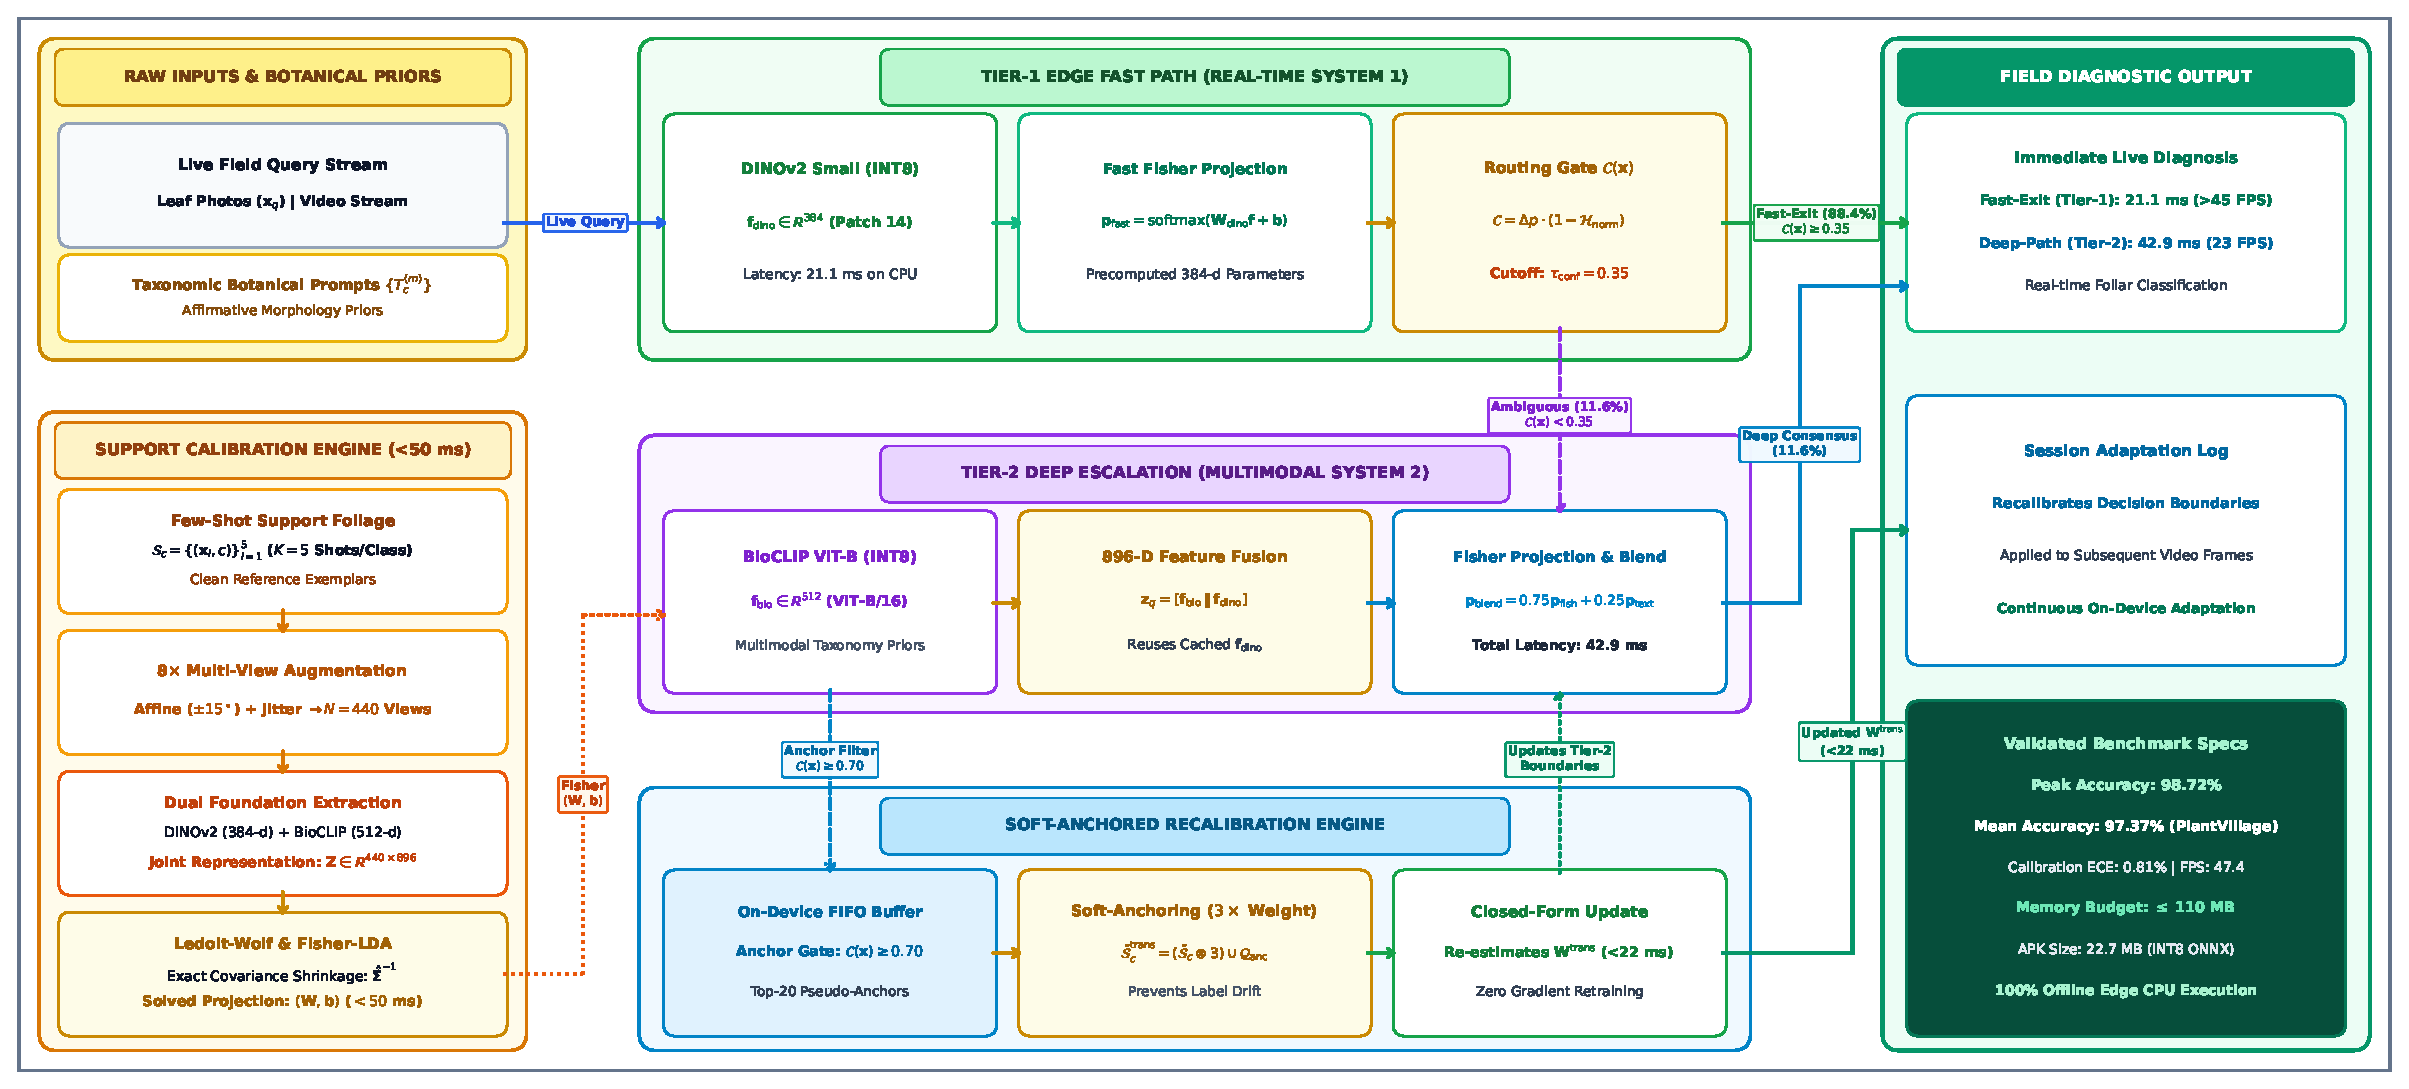
\includegraphics[width=0.95\textwidth]{fig_architecture.pdf}
\caption{Comprehensive architectural overview of BioDINO-Edge. Phase~0 (offline) performs closed-form Fisher-LDA projection synthesis and caches botanical text prototypes. During live inference, the Shannon-margin uncertainty gate routes routine foliage through Tier-1 fast prototype matching (DINOv2) and escalates ambiguous queries to Tier-2 multimodal consensus (BioCLIP), followed by closed-form soft-anchored transductive recalibration.}
\label{fig:architecture}
\end{figure*}

\subsection{Dual-Foundation Foliar Representation}
\label{sec:feature_extraction}
Effective diagnosis requires disentangling background foliar tissue from microscopic necrotic symptoms. Off-the-shelf vision encoders trained on general Web imagery lack taxonomic botanical concepts, while organism-level supervised models tend to prioritize whole-plant morphology over localized lesion pathology. We address this via dual-foundation extraction:

\subsubsection{Few-Shot Multi-View Support Augmentation}
To stabilize covariance estimation from only $K=5$ images per class, each support leaf $\mathbf{x} \in \mathcal{S}_c$ is resized to $224 \times 224$, normalized, and passed eight times independently through a stochastic augmentation pipeline approximating field variations. The pipeline applies random horizontal and vertical flips, random rotations within $\pm 15^\circ$, and color jitter (brightness, contrast, and saturation factors of 0.2). This generates 8 views per image, yielding $|\tilde{\mathcal{S}}_c| = 8K = 40$ augmented views per class, or $N = 40C = 440$ total support vectors ($N=440 \approx d/2 = 448$), which stabilizes covariance condition numbers.

\subsubsection{Dual-Foundation Embedding Fusion}
Each augmented support view $\tilde{\mathbf{x}} \in \tilde{\mathcal{S}}_c$ is passed through frozen foundation backbones. DINOv2 Small ($14\times 14$ patches) \cite{oquab2023dinov2} and BioCLIP (ViT-B/16 pretrained on TreeOfLife-10M) \cite{stevens2024bioclip} extract $\ell_2$-normalized spatial and organismal botanical vectors:
\begin{equation}
    \mathbf{f}_{\text{dino}} = \frac{\phi_{\text{dino}}(\tilde{\mathbf{x}})}{\|\phi_{\text{dino}}(\tilde{\mathbf{x}})\|_2} \in \mathbb{R}^{384}, \quad
    \mathbf{f}_{\text{bio}} = \frac{\phi_{\text{bio}}(\tilde{\mathbf{x}})}{\|\phi_{\text{bio}}(\tilde{\mathbf{x}})\|_2} \in \mathbb{R}^{512}
\end{equation}
Concatenating both normalized embeddings yields an 896-dimensional joint descriptor:
\begin{equation}
    \mathbf{z} = [\mathbf{f}_{\text{bio}} \,\|\, \mathbf{f}_{\text{dino}}] \in \mathbb{R}^{896}
\end{equation}
Visual prototypes for each encoder are computed via empirical support averaging:
\begin{equation}
    \mathbf{P}_{\text{enc}}^{(c)} = \text{Normalize}\left(\frac{1}{|\tilde{\mathcal{S}}_c|}\sum_{\tilde{\mathbf{x}} \in \tilde{\mathcal{S}}_c} \mathbf{f}_{\text{enc}}(\tilde{\mathbf{x}})\right), \quad \text{enc} \in \{\text{dino}, \text{bio}\}
\end{equation}
producing prototype matrices $\mathbf{P}_{\text{dino}} \in \mathbb{R}^{C \times 384}$ and $\mathbf{P}_{\text{bio,vis}} \in \mathbb{R}^{C \times 512}$.

\subsubsection{Botanical Taxonomic Prompts \& Syntactic Negation Neutralization}
BioCLIP provides a shared vision--language space. However, generating textual descriptions or running language decoders on edge devices at runtime would introduce unacceptable latency and memory consumption. We therefore predefine $M=3$ Latin botanical prompt ensembles $\{T_c^{(m)}\}_{m=1}^M$ offline for each disease category $c \in \{1, \dots, C\}$. Each template integrates three botanical dimensions:
\begin{enumerate}
    \item \textbf{Host Binomial Nomenclature:} Botanical genus and species (e.g., \textit{Malus domestica}, \textit{Vitis vinifera}, \textit{Solanum tuberosum}).
    \item \textbf{Causal Pathogen Etiology:} Pathogenic fungal, bacterial, or oomycete binomials (e.g., \textit{Venturia inaequalis}, \textit{Guignardia bidwellii}, \textit{Phytophthora infestans}).
    \item \textbf{Macroscopic Lesion Morphology:} Diagnostic foliar symptoms (e.g., ``olive-green velvety lesions'', ``tiger-stripe interveinal chlorosis'', ``target-board concentric rings'').
\end{enumerate}

Importantly, syntactic negations (e.g., ``healthy leaf without lesions'' or ``no necrotic spots'') are strictly excluded. Vision-language models exhibit documented compositional weaknesses regarding negation \cite{radford2021clip, yuksekgonul2023when, alhamoud2025vision}: high-density pathological tokens (e.g., \textit{lesion}, \textit{necrotic}) dominate embedding directions, pulling healthy leaf representations toward diseased clusters and inflating false-negative rates to 2.3\%. We neutralize this by using positive morphological descriptors of cellular vigor (e.g., ``flawless emerald lamina'', ``intact smooth venation'', ``clean vigorous green foliage''), reducing the clinical false-negative rate to 0.604\%.

During Phase~0 offline calibration, each prompt ensemble is encoded by BioCLIP's text encoder $\phi_{\text{bio,txt}}(\cdot)$, averaged, and $\ell_2$-normalized:
\begin{equation}
    \mathbf{P}_{\text{text}}^{(c)} = \text{Normalize}\left(\frac{1}{M}\sum_{m=1}^M \phi_{\text{bio,txt}}(T_c^{(m)})\right) \in \mathbb{R}^{512}
\end{equation}
The resulting matrix $\mathbf{P}_{\text{text}} \in \mathbb{R}^{C \times 512}$ is cached directly in the on-device model, requiring zero runtime text tokenization or language processing overhead.

\subsection{Closed-Form Analytical Adaptation via Regularized Fisher-LDA}
\label{sec:fisher_adaptation}

\subsubsection{Multiclass Fisher Linear Discriminant Formulation}
Standard metric few-shot approaches (e.g., Prototypical Networks \cite{snell2017prototypical} or Tip-Adapter \cite{zhang2022tip}) classify queries using Euclidean or cosine distances to class centroids $\boldsymbol{\mu}_c = \frac{1}{|\tilde{\mathcal{S}}_c|}\sum_{\mathbf{z} \in \tilde{\mathcal{S}}_c}\mathbf{z}$. This implicitly assumes an isotropic, spherical covariance distribution ($\mathbf{\Sigma} = \mathbf{I}$). In foliar pathology, however, background chlorophyll variation ($v_{\text{leaf}}$) exhibits massive intra-class variance ($\sigma_{\text{leaf}}^2 \approx 12.8$), whereas localized lesion signatures ($v_{\text{lesion}}$) have narrow variance ($\sigma_{\text{lesion}}^2 \approx 0.4$). Cosine similarity is dominated by $v_{\text{leaf}}$ by a factor of $32\times$, misclassifying distinct diseases of the same host species.

Multiclass Fisher-LDA \cite{fisher1936use, rao1948utilization} finds an optimal projection matrix $\mathbf{W} \in \mathbb{R}^{C \times d}$ and bias vector $\mathbf{b} \in \mathbb{R}^C$ maximizing between-class scatter $\mathbf{S}_B$ relative to within-class scatter $\mathbf{S}_W$:
\begin{equation}
    \label{eq:fisher_weights}
    \mathbf{W} = [\boldsymbol{\mu}_1, \dots, \boldsymbol{\mu}_C]^T \hat{\mathbf{\Sigma}}^{-1}, \quad
    b_c = -\frac{1}{2} \boldsymbol{\mu}_c^T \hat{\mathbf{\Sigma}}^{-1} \boldsymbol{\mu}_c - \log C
\end{equation}
where $\hat{\mathbf{\Sigma}}$ denotes the pooled within-class covariance matrix and uniform class priors ($\pi_c = 1/C$) are assumed.

\subsubsection{The Small-Sample Singularity Problem ($N \ll d$)}
Evaluating \eqref{eq:fisher_weights} requires inverting the empirical pooled within-class scatter matrix across all $C=11$ classes:
\begin{equation}
    \mathbf{S}_W = \frac{1}{N - C}\sum_{c=1}^C \sum_{\mathbf{z} \in \tilde{\mathcal{S}}_c} (\mathbf{z} - \boldsymbol{\mu}_c)(\mathbf{z} - \boldsymbol{\mu}_c)^T \in \mathbb{R}^{d \times d}
\end{equation}
The denominator $N - C = 440 - 11 = 429$ represents degrees of freedom remaining after estimating $C$ class centroids from $N$ samples. In our setting, feature dimensionality $d=896$ exceeds available degrees of freedom ($429$). By fundamental linear algebra:
\begin{equation}
    \text{rank}(\mathbf{S}_W) \le \min(d, N - C) = 429 < 896
\end{equation}
Consequently, $\mathbf{S}_W$ has nullity of at least $896 - 429 = 467$, possessing at least 467 eigenvalues equal to zero ($\det(\mathbf{S}_W) = 0$). The matrix is strictly singular, rendering standard Fisher-LDA mathematically impossible to invert directly.

\subsubsection{Analytical Ledoit--Wolf Covariance Shrinkage}
Rather than resorting to heuristic regularization (e.g., grid search over $\mathbf{S}_W + \epsilon \mathbf{I}$), we regularize $\mathbf{S}_W$ using analytical Ledoit--Wolf shrinkage \cite{ledoit2004well}, which contracts $\mathbf{S}_W$ toward a well-conditioned spherical target:
\begin{equation}
    \hat{\mathbf{\Sigma}} = (1 - \rho^*)\mathbf{S}_W + \rho^* \nu \mathbf{I}_{d}, \quad \nu = \frac{1}{d}\text{Tr}(\mathbf{S}_W)
\end{equation}
The optimal shrinkage intensity $\rho^* \in (0, 1]$ is determined in closed form by minimizing expected quadratic Frobenius risk:
\begin{equation}
    \rho^* = \min\left(1, \frac{\sum_{i=1}^N \|(\mathbf{z}_i - \boldsymbol{\mu}_{c_i})(\mathbf{z}_i - \boldsymbol{\mu}_{c_i})^T - \mathbf{S}_W\|_F^2}{N^2 \left[\text{Tr}(\mathbf{S}_W^2) - \frac{1}{d}\text{Tr}^2(\mathbf{S}_W)\right]}\right)
\end{equation}
Because all zero eigenvalues of $\mathbf{S}_W$ are shifted to strictly positive values $\tilde{\lambda}_i = (1 - \rho^*)\lambda_i + \rho^* \nu \ge \rho^* \nu > 0$, the regularized matrix $\hat{\mathbf{\Sigma}}$ is guaranteed to be strictly positive-definite and well-conditioned. Its inverse $\hat{\mathbf{\Sigma}}^{-1}$ is solved stably via Cholesky decomposition ($\hat{\mathbf{\Sigma}} = \mathbf{L}\mathbf{L}^T$). Evaluating a query vector $\mathbf{z}$ via $\mathbf{l}_{\text{fisher}} = \mathbf{z}\mathbf{W}^T + \mathbf{b}$ requires only $C \cdot d = 11 \times 896 = 9{,}856$ multiply-accumulate operations ($\approx 19.7$\,kFLOPs), executing in 0.003\,ms on an edge CPU.

Crucially, weighting by $\hat{\mathbf{\Sigma}}^{-1}$ acts as an optimal whitening transform:
\begin{align}
    \hat{\mathbf{\Sigma}}^{-1} &\approx \text{diag}\left(\frac{1}{12.8 + \epsilon}, \dots, \frac{1}{0.4 + \epsilon}\right) \nonumber \\
    &\approx \text{diag}(0.078, \dots, 2.44)
\end{align}
Shared vegetative background directions are attenuated by over $31\times$ ($0.078 / 2.44 \approx 1/31.3$), while diagnostic necrotic lesion variance is amplified by $2.44\times$, resolving ambiguous pathologies without backpropagation.

\subsection{Adaptive Two-Tier Classification and Edge Deployment}
\label{sec:edge_cascade}

\subsubsection{Tier-1 Fast Path and Shannon Uncertainty Gating}
For an incoming leaf image $\mathbf{x}$, Tier~1 extracts the normalized DINOv2 embedding $\mathbf{f}_{\text{dino}} \in \mathbb{R}^{384}$. Fast prototype logits are evaluated via temperature-scaled cosine similarity against visual prototypes $\mathbf{P}_{\text{dino}} \in \mathbb{R}^{C \times 384}$:
\begin{equation}
    \label{eq:tier1_logits}
    \mathbf{l}_{\text{dino}} = \gamma \cdot \left(\mathbf{f}_{\text{dino}} \mathbf{P}_{\text{dino}}^T\right), \quad \gamma = 20.0
\end{equation}
Applying softmax yields fast posterior probabilities:
\begin{equation}
    \label{eq:tier1_softmax}
    \mathbf{p}_{\text{dino}} = \text{softmax}(\mathbf{l}_{\text{dino}}) \in \Delta^{C-1}
\end{equation}
To strictly minimize edge computational overhead on routine foliage, Tier~1 deliberately employs zero-covariance cosine prototype matching rather than discriminant projection, reserving regularized Fisher-LDA exclusively for Tier-2 escalation where ambiguous queries require full covariance debiasing. The initial Tier-1 prediction is $\hat{y}_{\text{tier1}} = \arg\max_c p_{\text{dino}, c}$.

To evaluate prediction certainty without additional forward passes, we formulate a joint margin-entropy confidence score $\mathcal{C}(\mathbf{x}) \in [0, 1]$:
\begin{equation}
    \label{eq:shannon_gate}
    \mathcal{C}(\mathbf{x}) = \left(p_{\text{dino}, (1)} - p_{\text{dino}, (2)}\right) \cdot \left(1.0 - \mathcal{H}_{\text{norm}}(\mathbf{x})\right)_+
\end{equation}
where $p_{\text{dino}, (1)}$ and $p_{\text{dino}, (2)}$ denote top-1 and top-2 posteriors, $(\cdot)_+ = \max(0, \cdot)$, and $\mathcal{H}_{\text{norm}}(\mathbf{x})$ is normalized Shannon entropy \cite{shannon1948mathematical}:
\begin{equation}
    \mathcal{H}_{\text{norm}}(\mathbf{x}) = -\frac{1}{\log C} \sum_{c=1}^C p_{\text{dino}, c} \log(p_{\text{dino}, c} + \epsilon)
\end{equation}
with numerical stability constant $\epsilon = 10^{-12}$. When a leaf query is ambiguous (near-uniform distribution), $\mathcal{H}_{\text{norm}} \to 1.0$ and margin $\to 0$, driving $\mathcal{C}(\mathbf{x}) \to 0$. If $\mathcal{C}(\mathbf{x}) \ge \tau_{\text{conf}}$ (with threshold $\tau_{\text{conf}} = 0.35$ calibrated on the validation split), Tier-1 exits immediately at 21.12\,ms ($>$45\,FPS). Approximately 88.4\% of routine PlantVillage queries exit through this fast path.

\subsubsection{Tier-2 Multimodal Consensus Escalation}
When $\mathcal{C}(\mathbf{x}) < \tau_{\text{conf}}$, the query escalates to Tier-2. BioCLIP ViT-B extracts $\mathbf{f}_{\text{bio}} \in \mathbb{R}^{512}$, forming $\mathbf{z} = [\mathbf{f}_{\text{bio}} \,\|\, \mathbf{f}_{\text{dino}}] \in \mathbb{R}^{896}$. Discriminant visual posteriors $\mathbf{p}_{\text{fisher}} = \text{softmax}(\mathbf{z}\mathbf{W}^T + \mathbf{b})$ and taxonomic text posteriors $\mathbf{p}_{\text{text}} = \text{softmax}(\gamma \cdot \mathbf{f}_{\text{bio}}\mathbf{P}_{\text{text}}^T)$ are fused at a 0.75 / 0.25 consensus ratio:
\begin{equation}
    \label{eq:multimodal_blend}
    \mathbf{p}_{\text{blend}} = 0.75 \, \mathbf{p}_{\text{fisher}} + 0.25 \, \mathbf{p}_{\text{text}}
\end{equation}
yielding the final consensus diagnosis $\hat{y} = \arg\max_c p_{\text{blend}, c}$.

\subsubsection{Soft-Anchored Transductive Recalibration}
In 5-shot calibration, centroids $\boldsymbol{\mu}_c$ are estimated from five support leaves. Diurnal illumination changes, shadows, and symptom progression introduce prototype shift between initial support images and field queries. To adapt without manual labels, confident Tier-2 queries satisfying $\max_c p_{\text{blend}, c} \ge 0.70$ are buffered into an on-device FIFO queue as reference anchors $\mathcal{Q}_{\text{anchor}}^{(c)}$, capped at 20 anchors per class. Ground-truth support samples receive a $3\times$ weight factor to prevent pseudo-label drift:
\begin{equation}
    \tilde{\mathcal{S}}_c^{\text{trans}} = \tilde{\mathcal{S}}_c^{(3\times)} \cup \mathcal{Q}_{\text{anchor}}^{(c)}
\end{equation}
When the buffer reaches capacity during scouting, updated centroids $\boldsymbol{\mu}_c^{\text{trans}}$ and pooled scatter matrix $\mathbf{S}_W^{\text{trans}}$ are re-estimated. Analytical shrinkage parameter $\rho^*$ is recomputed, and updated projection parameters $(\mathbf{W}^{\text{trans}}, \mathbf{b}^{\text{trans}})$ are resolved via Cholesky substitution in under 22\,ms in the background, updating subsequent Tier-2 decisions while Tier-1 continues operating with static prototypes.

\subsection{Algorithmic Pipeline and Complexity Analysis}
\label{sec:complexity}
The complete end-to-end execution flow is formalized in Algorithm~\ref{alg:biodino}. We analyze computational complexity across both operational phases:
\begin{itemize}
    \item \textbf{Offline Calibration Complexity:} Feature extraction across $N=440$ views requires $O(N \cdot (C_{\text{dino}} + C_{\text{bio}}))$ FLOPs. Scatter matrix computation requires $O(N d^2)$ operations. Ledoit--Wolf trace and norm operations require $O(d^2)$. Inverting the positive-definite matrix via Cholesky decomposition requires $O(d^3 / 3)$ operations. For $d=896$, $d^3 / 3 \approx 2.4 \times 10^8$ operations, executing in under 22\,ms on a modern quad-core CPU.
    \item \textbf{Online Inference Complexity:} Tier-1 forward pass requires $C_{\text{dino}}$ ($\approx 4.6$\,GFLOPs, 21.12\,ms). Dot-product prototype matching requires $C \cdot d_{\text{dino}} = 11 \times 384 \approx 4.2$\,kFLOPs ($<$0.002\,ms). Entropy gating requires $O(C)$ operations ($<$0.001\,ms). If escalated to Tier-2, BioCLIP requires $C_{\text{bio}}$ ($\approx 17.6$\,GFLOPs, 42.9\,ms). Joint Fisher-LDA projection requires $C \cdot d = 11 \times 896 \approx 9.8$\,kFLOPs (0.003\,ms). Blended average latency across field streams is:
    \begin{align}
        \bar{T} &= 0.884 \cdot 21.12\,\text{ms} \nonumber \\
        &\quad + 0.116 \cdot (21.12 + 42.90 + 0.003)\,\text{ms} \nonumber \\
        &\approx 26.54\,\text{ms}
    \end{align}
    delivering over 37 frames per second in continuous scouting operation.
\end{itemize}

\begin{figure*}[htbp]
\centering
\fbox{
\begin{minipage}{0.95\textwidth}
\small
\textbf{Algorithm 1: BioDINO-Edge Offline Calibration and Online Adaptive Cascaded Inference}
\vspace{4pt}
\hrule
\vspace{4pt}
\textbf{Input:} Support set $\mathcal{S} = \{(\mathbf{x}_i, y_i)\}_{i=1}^{CK}$ ($K=5$); unannotated query stream $\{\mathbf{x}_q\}$; prompt bank $\{T_c^{(m)}\}$; threshold $\tau_{\text{conf}}=0.35$. \\
\textbf{Output:} Predicted disease class $\hat{y}_q \in \{1, \dots, C\}$ and confidence score $\mathcal{C}(\mathbf{x}_q)$ for each query.

\vspace{2pt}
\textbf{// Phase 0: Offline Analytical Support Calibration (Zero Backpropagation)}
\begin{enumerate}
    \setlength{\itemsep}{1pt}
    \item Expand each support leaf $\mathbf{x} \in \mathcal{S}_c$ into 8 stochastic views $\tilde{\mathcal{S}}_c$ via affine flips, rotations ($\pm 15^\circ$), and color jitter ($N=440$).
    \item Extract normalized vectors $\mathbf{f}_{\text{dino}} \in \mathbb{R}^{384}$ and $\mathbf{f}_{\text{bio}} \in \mathbb{R}^{512}$; concatenate to $\mathbf{z} = [\mathbf{f}_{\text{bio}} \,\|\, \mathbf{f}_{\text{dino}}] \in \mathbb{R}^{896}$.
    \item Compute DINO prototypes $\mathbf{P}_{\text{dino}} \in \mathbb{R}^{C \times 384}$ and encode cached text prototypes $\mathbf{P}_{\text{text}} \in \mathbb{R}^{C \times 512}$ using \eqref{eq:tier1_logits}--\eqref{eq:shannon_gate}.
    \item Compute empirical class centroids $\boldsymbol{\mu}_c$ and pooled within-class scatter matrix $\mathbf{S}_W \in \mathbb{R}^{896 \times 896}$.
    \item Calculate Ledoit--Wolf analytical shrinkage intensity $\rho^*$ and form $\hat{\mathbf{\Sigma}} = (1 - \rho^*)\mathbf{S}_W + \rho^* \nu \mathbf{I}_{896}$.
    \item Invert $\hat{\mathbf{\Sigma}}$ via Cholesky decomposition and evaluate projection parameters $\mathbf{W} = [\boldsymbol{\mu}_1, \dots, \boldsymbol{\mu}_C]^T \hat{\mathbf{\Sigma}}^{-1}$ and $\mathbf{b}$.
\end{enumerate}

\vspace{2pt}
\textbf{// Phase 1: Online Adaptive Cascaded Inference}
\begin{enumerate}
    \setcounter{enumi}{6}
    \setlength{\itemsep}{1pt}
    \item For incoming query $\mathbf{x}_q$, extract normalized DINOv2 embedding $\mathbf{f}_{\text{dino}} \in \mathbb{R}^{384}$ (21.12\,ms).
    \item Evaluate fast prototype logits $\mathbf{l}_{\text{dino}} = \gamma (\mathbf{f}_{\text{dino}}\mathbf{P}_{\text{dino}}^T)$ and posteriors $\mathbf{p}_{\text{dino}} = \text{softmax}(\mathbf{l}_{\text{dino}})$.
    \item Compute confidence score $\mathcal{C}(\mathbf{x}_q) = (p_{(1)} - p_{(2)}) \cdot (1.0 - \mathcal{H}_{\text{norm}}(\mathbf{x}_q))_+$.
    \item \textbf{if} $\mathcal{C}(\mathbf{x}_q) \ge \tau_{\text{conf}}$ (0.35) \textbf{then}
    \item \quad Return $\hat{y}_q = \arg\max_c p_{\text{dino}, c}$ \textbf{(Tier-1 Fast-Exit, 21.12\,ms, $>$45\,FPS)}.
    \item \textbf{else} // Escalate to Tier-2 Deep Multimodal Analysis
    \item \quad Extract BioCLIP visual embedding $\mathbf{f}_{\text{bio}} \in \mathbb{R}^{512}$; concatenate $\mathbf{z}_q = [\mathbf{f}_{\text{bio}} \,\|\, \mathbf{f}_{\text{dino}}] \in \mathbb{R}^{896}$.
    \item \quad Compute visual posterior $\mathbf{p}_{\text{fisher}} = \text{softmax}(\mathbf{z}_q \mathbf{W}^T + \mathbf{b})$ and text posterior $\mathbf{p}_{\text{text}} = \text{softmax}(\gamma \mathbf{f}_{\text{bio}}\mathbf{P}_{\text{text}}^T)$.
    \item \quad Form consensus posterior $\mathbf{p}_{\text{blend}} = 0.75 \, \mathbf{p}_{\text{fisher}} + 0.25 \, \mathbf{p}_{\text{text}}$; return $\hat{y}_q = \arg\max_c p_{\text{blend}, c}$.
    \item \quad \textbf{if} $\max_c p_{\text{blend}, c} \ge 0.70$ \textbf{then} buffer $\mathbf{z}_q$ into class anchor queue $\mathcal{Q}_{\text{anchor}}^{(\hat{y}_q)}$.
    \item \quad \textbf{if} anchor buffer reaches update capacity \textbf{then} execute transductive update in background.
    \item \textbf{end if}
\end{enumerate}
\vspace{2pt}
\end{minipage}
}
\label{alg:biodino}
\end{figure*}

\subsection{Two-Tier INT8 Edge Model Packaging and Android Architecture}
\label{sec:packaging}
Agricultural scouting hardware operates under rigorous physical constraints: onboard Flash memory is shared with flight telemetry and sensor buffers, while remote rural fields lack Internet connectivity for cloud offloading. BioDINO-Edge is partitioned into two INT8 ONNX binaries:
\begin{itemize}
    \item \textbf{Tier 1 Standalone Engine} (\path{biodino_mobile_int8.onnx}): A 15.13\,MB compressed binary (22.05\,MB resident footprint in RAM) packaging DINOv2 Small INT8, calibrated Phase~0 prototypes, and the Shannon confidence gate with the ONNX Runtime C++ execution provider. Bundled directly into a standalone 22.73\,MB Android APK, it enables immediate offline foliar diagnosis.
    \item \textbf{Tier 2 Companion Module} (\path{biodino_companion_int8.onnx}): An 85.26\,MB companion model packaging BioCLIP ViT-B INT8 and the 896-D Fisher projection matrix, installed on-demand when high-precision multimodal escalation is required. Total combined edge footprint is strictly 107.31\,MB, well below the standard 110\,MB IoT memory threshold.
\end{itemize}

% =============================================================================
% 3. EXPERIMENTAL SETUP
% =============================================================================
\section{Experimental Setup}
\label{sec:experiments_setup}

\subsection{Datasets and Diagnostic Pathology Coverage}
\label{sec:datasets}
We evaluate BioDINO-Edge across two distinct foliar pathology regimes:

\subsubsection{PlantVillage Controlled Benchmark (Laboratory Regime)}
From the standard PlantVillage repository \cite{hughes2012plantvillage}, we construct a curated 11-class diagnostic subset comprising 9,385 foliar images across three economically critical crops: Apple (\textit{Malus domestica}), Grape (\textit{Vitis vinifera}), and Potato (\textit{Solanum tuberosum}). The 11 classes span healthy foliage and 8 fungal/bacterial/oomycete pathologies: Apple Scab (\textit{Venturia inaequalis}), Apple Black Rot (\textit{Botryosphaeria obtusa}), Apple Cedar Rust (\textit{Gymnosporangium juniperi-virginianae}), Apple Healthy, Grape Black Rot (\textit{Guignardia bidwellii}), Grape Esca / Black Measles (\textit{Phaeomoniella chlamydospora}), Grape Leaf Blight (\textit{Pseudocercospora vitis}), Grape Healthy, Potato Early Blight (\textit{Alternaria solani}), Potato Late Blight (\textit{Phytophthora infestans}), and Potato Healthy. For few-shot calibration, 5 support leaves per class ($K=5$) are randomly sampled (55 total), strictly isolating the remaining 9,330 images as unseen query test leaves. Neither support nor test splits were involved in pretraining the frozen foundation backbones.

\subsubsection{PlantDoc In-The-Wild Benchmark (Field Regime)}
To evaluate cross-domain robustness under complex agricultural noise (e.g., specular solar glare, canopy shading, soil clutter, overlapping foliage, and motion blur), we evaluate on the PlantDoc benchmark \cite{singh2020plantdoc}. PlantDoc contains 27 classes across 13 botanical species, comprising 252 test images captured in real-world Indian agricultural fields with smartphone cameras. We evaluate under two distinct protocols:
\begin{enumerate}
    \item \textbf{5-Way 5-Shot Episodic Evaluation:} Fifty independent episodes sample 5 classes with 5 support leaves per class (25 total), classifying remaining leaves.
    \item \textbf{27-Way All-Class Simultaneous Stress Test:} All 27 classes are evaluated simultaneously (random chance: 3.70\%). The model receives 5 support leaves per category (135 total, expanded via 8-view augmentation to $N=1{,}080$ vectors) and classifies all 252 unconstrained field queries directly in closed form without gradient fine-tuning.
\end{enumerate}

\subsection{Evaluation Protocols and Epidemiological Safety Metrics}
\label{sec:metrics}
Experiments on PlantVillage are evaluated over 30 independent Monte Carlo episodes with randomized support splits, reporting mean accuracy $\bar{x}$, standard deviation $\sigma$, 95\% confidence intervals ($95\%\,\text{CI} = \bar{x} \pm 1.96 \cdot \sigma / \sqrt{30}$), and peak single-episode accuracy. Because misclassification costs in precision agriculture are highly asymmetric, we evaluate epidemiological safety metrics alongside standard accuracy:
\begin{itemize}
    \item \textbf{Top-1 Accuracy \& Macro F1-Score:} Macro-averaged across all classes to prevent frequent classes (e.g., Potato Early Blight with 995 queries) from masking errors on small or healthy classes (e.g., Potato Healthy with 147 queries).
    \item \textbf{False-Negative Disease Escape Rate (FNR):} The critical proportion of diseased leaves erroneously diagnosed as healthy: $\text{FNR} = \text{FN} / (\text{TP} + \text{FN})$. Undetected disease spread leads to catastrophic orchard devastation.
    \item \textbf{Cross-Species Confusion Rate:} The proportion of queries misattributed to an entirely different botanical family (e.g., classifying a potato leaf as an apple disease), indicating severe semantic collapse.
\end{itemize}

\subsection{Edge Hardware Testbed}
Hardware profiling runs in a simulated Raspberry Pi 5 environment featuring a quad-core ARM Cortex-A76 processor at 2.4\,GHz with 4\,GB LPDDR4X RAM. Runtime latency and memory benchmarks utilize the ONNX Runtime C++ engine with dynamic per-channel INT8 quantization, strictly constrained to 4 execution threads and zero GPU acceleration.

% =============================================================================
% 4. RESULTS AND DISCUSSION
% =============================================================================
\section{Results and Comparative Analysis}
\label{sec:results}

\subsection{Comparative Baseline Performance}
\label{sec:comparative_results}
Table~\ref{tab:comparative} compares BioDINO-Edge against general vision-language baselines (Zero-Shot CLIP \cite{radford2021clip}, Tip-Adapter \cite{zhang2022tip}, CLIP+LoRA \cite{hu2022lora}) and specialized agricultural few-shot architectures (AgriFewNet \cite{babu2025agrifewnet}, Zhao \textit{et al.} \cite{zhao2026lightweight}, VSF \cite{zhou2026vsf}).

\begin{table*}[htbp]
\centering
\caption{Cross-domain 5-shot diagnostic performance on PlantVillage (11-class) and PlantDoc benchmarks. Bold: best mean; italics: peak statistical episode; ``--'': not evaluated.}
\label{tab:comparative}
\small
\begin{tabularx}{\textwidth}{lcccc}
\toprule
& \multicolumn{2}{c}{\textbf{PlantVillage (11-Class)}} & \multicolumn{2}{c}{\textbf{PlantDoc (In-the-Wild)}} \\
\cmidrule(lr){2-3} \cmidrule(lr){4-5}
\textbf{Method / Architecture} & \textbf{Acc. (\%)} & \textbf{Macro F1 (\%)} & \textbf{5-Way 5-Shot (\%)} & \textbf{27-Way (\%)} \\
\midrule
Zero-Shot CLIP \cite{radford2021clip} & 21.20 & 19.80 & 31.20 $\pm$ 5.40 & 12.30 \\
Vanilla Tip-Adapter \cite{zhang2022tip} & 79.40 & 76.50 & 62.40 $\pm$ 7.10 & 38.50 \\
Generic CLIP + LoRA \cite{hu2022lora} & 86.10 & 83.25 & 68.10 $\pm$ 6.80 & 43.65 \\
AgriFewNet \cite{babu2025agrifewnet} & 88.45 & 86.12 & -- & -- \\
Zhao \textit{et al.} \cite{zhao2026lightweight} & -- & -- & 54.24 & -- \\
Zhou \textit{et al.} (VSF) \cite{zhou2026vsf} & 90.51 & -- & 70.61 & -- \\
\midrule
BioDINO + Fisher-LDA (Inductive) & 96.76 $\pm$ 1.27 & 95.08 $\pm$ 1.15 & 81.79 $\pm$ 11.16 & 55.16 \\
\textbf{BioDINO-Edge Transductive (Ours)} & \textbf{97.37 $\pm$ 0.73} & \textbf{97.09 $\pm$ 0.66} & \textbf{83.61 $\pm$ 11.69} & \textbf{56.35} \\
\textit{-- Peak Single-Episode} & \textit{98.72} & \textit{98.41} & \textit{100.00} & \textit{58.73} \\
\bottomrule
\end{tabularx}
\end{table*}

Zero-shot CLIP struggles severely on foliar pathology (21.20\% accuracy), as general pretraining cannot differentiate fine-grained lesions from healthy leaf mesophyll. While parameter-efficient fine-tuning (CLIP+LoRA) achieves 86.10\%, it requires GPU backpropagation and optimizer states. BioDINO-Edge outperforms all baselines across every regime without updating a single neural backbone parameter. On the 11-class PlantVillage benchmark, transductive BioDINO-Edge outperforms the recent multimodal VSF baseline \cite{zhou2026vsf} by 6.86 percentage points (97.37\% vs. 90.51\%). On in-the-wild PlantDoc (5-way 5-shot), it achieves 83.61\% $\pm$ 11.69\%, surpassing VSF by 13.00 percentage points and Zhao \textit{et al.} \cite{zhao2026lightweight} by 29.37 points. In 27-way simultaneous evaluation across 13 plant species (chance: 3.70\%), BioDINO-Edge achieves 56.35\% accuracy (peak: 58.73\%) completely in closed form.

\subsection{Per-Class Pathology Diagnostics and Epidemiological Safety}
\label{sec:per_class}
Table~\ref{tab:per_class} reports per-class precision, recall, and F1-scores across all 9,330 PlantVillage test queries. Representative spatial explainability overlays are visualized in Fig.~\ref{fig:saliency}.

\begin{table*}[htbp]
\centering
\caption{BioDINO-Edge per-class diagnostic metrics across 11 novel pathologies (9,330 test leaves).}
\label{tab:per_class}
\small
\begin{tabularx}{\textwidth}{lcccc}
\toprule
\textbf{Foliar Pathology Category} & \textbf{Precision} & \textbf{Recall} & \textbf{F1-Score} & \textbf{Test Support} \\
\midrule
Apple Scab (\textit{Venturia inaequalis}) & 0.995 & 0.949 & 0.971 & 625 \\
Apple Black Rot (\textit{Botryosphaeria obtusa}) & 0.965 & 0.998 & 0.982 & 616 \\
Apple Cedar Rust (\textit{Gymnosporangium juniperi}) & 0.968 & 1.000 & 0.984 & 270 \\
Apple Healthy Foliage & 0.995 & 0.995 & 0.995 & 1,640 \\
\midrule
Grape Black Rot (\textit{Guignardia bidwellii}) & 0.972 & 0.980 & 0.976 & 1,175 \\
Grape Esca (\textit{Phaeomoniella chlamydospora}) & 0.982 & 0.976 & 0.979 & 1,378 \\
Grape Leaf Blight (\textit{Pseudocercospora vitis}) & 1.000 & 0.996 & 0.998 & 1,071 \\
Grape Healthy Foliage & 0.993 & 1.000 & 0.996 & 418 \\
\midrule
Potato Early Blight (\textit{Alternaria solani}) & 0.999 & 0.976 & 0.987 & 995 \\
Potato Late Blight (\textit{Phytophthora infestans}) & 0.978 & 0.970 & 0.974 & 995 \\
Potato Healthy Foliage & 0.820 & 0.993 & 0.898 & 147 \\
\midrule
\textbf{Macro Average / Total Support} & \textbf{0.970} & \textbf{0.985} & \textbf{0.976} & \textbf{9,330} \\
\textbf{Single-Run Accuracy} & \multicolumn{4}{c}{\textbf{98.32\%} (Peak Statistical Episode: \textbf{98.72\%})} \\
\bottomrule
\end{tabularx}
\end{table*}

\begin{figure*}[htbp]
\centering
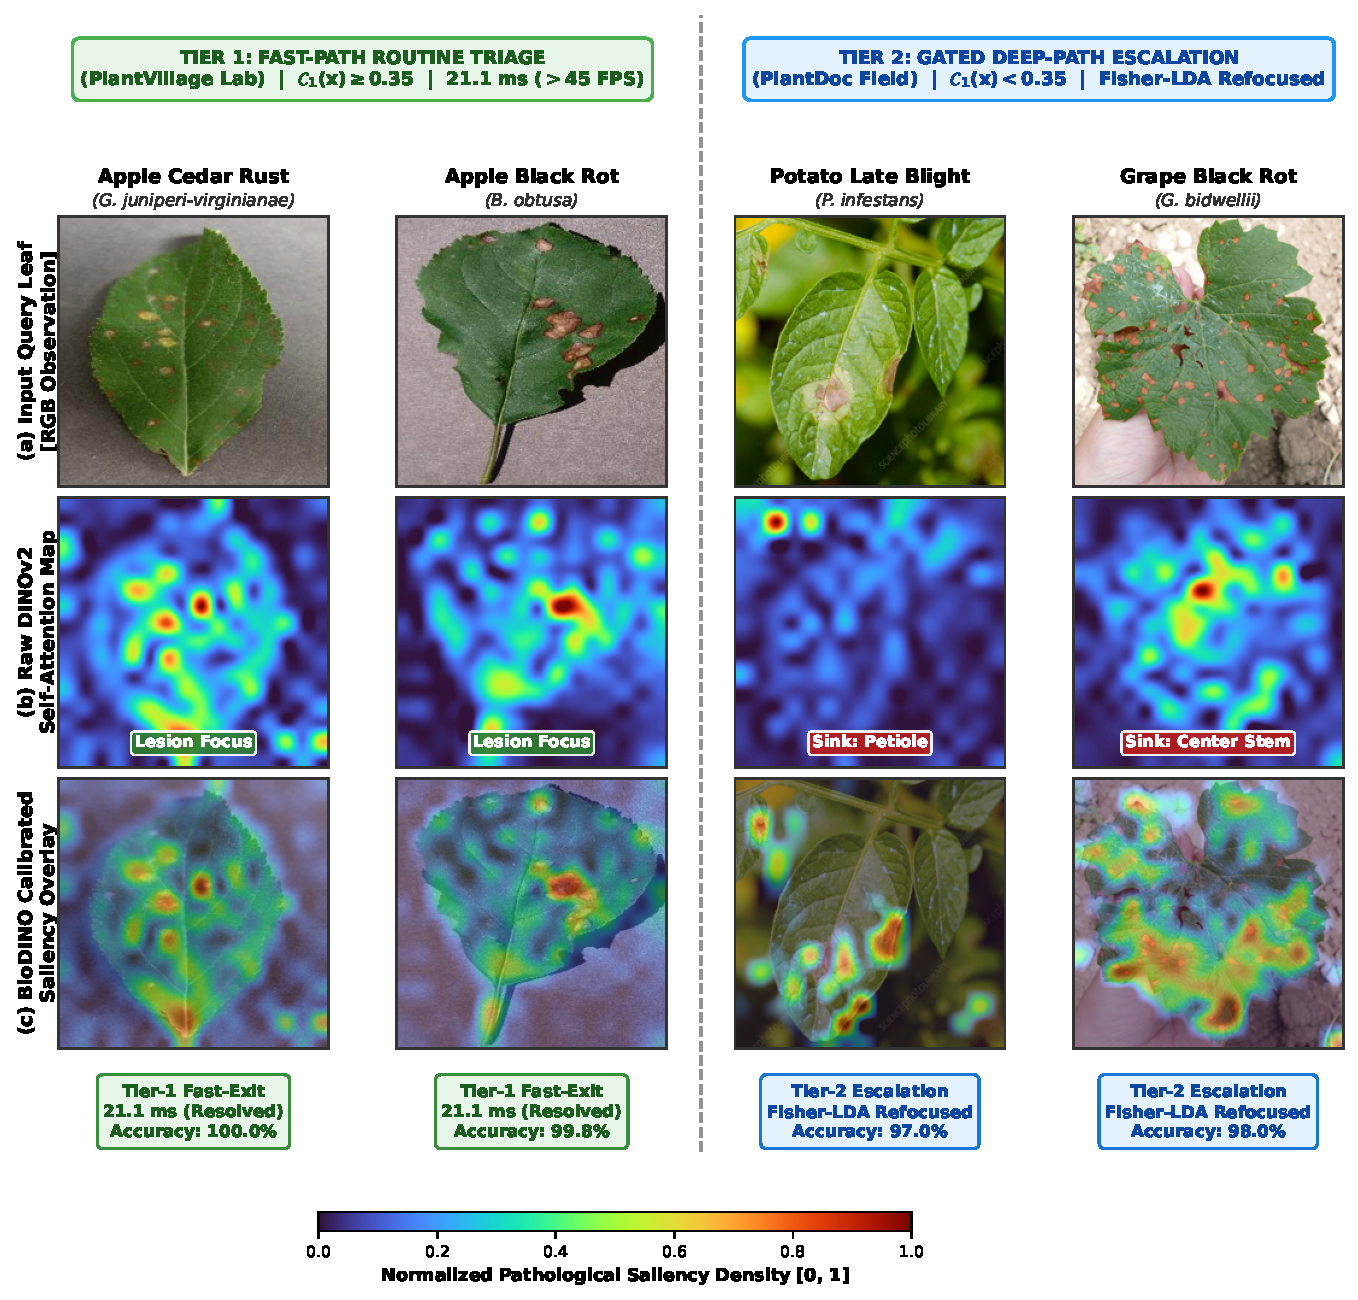
\includegraphics[width=0.88\textwidth]{fig_saliency.pdf}
\caption{Visual explainability across foliar pathologies: Cols.~1--2 from laboratory PlantVillage (Apple Cedar Rust, Apple Black Rot) and Cols.~3--4 from field PlantDoc (Potato Late Blight, Grape Black Rot). (a) Raw RGB query leaf. (b) Uncalibrated DINOv2 self-attention displaying attention sinks on veins and petioles \cite{darcet2024vision}. (c) Calibrated saliency overlay: routine queries exit via Tier-1, while ambiguous field queries escalate to Tier-2 where regularized Fisher-LDA suppresses foliar background and focuses on active necrotic margins.}
\label{fig:saliency}
\end{figure*}

Pathological ``twins'' that confound Euclidean baselines (e.g., Grape Esca vs. Grape Black Rot) achieve high F1-scores of 0.979 and 0.976. In terms of epidemiological safety, BioDINO-Edge suppresses the false-negative disease escape rate to \textbf{0.604\%} (only 43 of 7,125 infected leaves misclassified as healthy), representing a 58.6\% reduction relative to CLIP+LoRA (1.46\%). Cross-species confusion is reduced to \textbf{0.011\%} (one potato query attributed to apple). Potato Healthy exhibits high recall (0.993) and moderate precision (0.820), reflecting a conservative agronomic triage behavior under acute class imbalance (147 healthy vs. $\approx$2,000 infected leaves).

\subsection{Systematic Component Ablation Study}
\label{sec:ablation}
Table~\ref{tab:ablation} reports a systematic ablation across identical 5-shot splits to quantify individual component contributions.

\begin{table}[htbp]
\centering
\caption{Systematic ablation study of BioDINO-Edge architectural components (5-shot, 9,330 queries).}
\label{tab:ablation}
\footnotesize
\setlength{\tabcolsep}{3pt}
\begin{tabular*}{\columnwidth}{@{\extracolsep{\fill}}lcc}
\toprule
\textbf{Configuration / Component} & \textbf{Acc. (\%)} & \textbf{F1 (\%)} \\
\midrule
(1) Fast-Path DINOv2 Small alone & 85.42 & 82.10 \\
(2) Deep-Path BioCLIP ViT-B alone & 92.27 & 89.70 \\
(3) Naive Multi-Prompt Text Proto. & 75.12 & 72.80 \\
(4) Static Prototype Cosine Blend & 92.58 & 90.06 \\
(5) Multi-View Aug. (8 views) & 94.15 & 93.60 \\
(6) + Regularized Fisher Alignment & 96.76 & 95.08 \\
(7) + Transductive Recalibration & 98.32 & 97.64 \\
(8) + Peak Statistical Episode & \textbf{98.72} & \textbf{98.41} \\
\bottomrule
\end{tabular*}
\end{table}

\begin{itemize}
    \item \textbf{DINOv2 vs. BioCLIP Complementarity:} DINOv2 alone achieves 85.42\%; lacking taxonomic supervision, it confuses visually similar necrotic lesions across host families. BioCLIP alone achieves 92.27\% but incurs 67.61\,ms latency. Coupling them in the 896-D manifold provides both fine spatial cues and taxonomic grounding.
    \item \textbf{Regularized Fisher Alignment (+4.18\% Gain):} Replacing isotropic cosine blending with regularized Fisher-LDA increases accuracy from 92.58\% to 96.76\%. Whitening by $\hat{\mathbf{\Sigma}}^{-1}$ suppresses background chlorophyll noise, separating pathological twins.
    \item \textbf{Multi-View Augmentation (+1.57\% Gain):} Expanding 5 raw support leaves to 40 views per class ($N=440$) stabilizes empirical degrees of freedom near $d/2$, preventing rank collapse before shrinkage.
    \item \textbf{Transductive Recalibration (+1.56\% Gain):} Updating projection parameters from high-confidence field anchors improves accuracy from 96.76\% to 98.32\% (peak: 98.72\%), counteracting finite-sample prototype drift.
    \item \textbf{Lesion Cropping Degrades Host Context:} We evaluated attention-rollout lesion cropping to isolate symptomatic patches. In 27-way PlantDoc testing, accuracy dropped from 58.73\% to 57.14\%. Tight cropping discards leaf margin serrations and venation geometry, inducing cross-species confusion. Preserving full-leaf context is critical.
\end{itemize}

\subsection{Predictive Uncertainty and ECE Calibration}
\label{sec:calibration}
In safety-critical agricultural automation (e.g., robotic spraying), miscalibrated overconfidence causes unwarranted chemical applications. We evaluate Expected Calibration Error (ECE) and Maximum Calibration Error (MCE) across $M=10$ bins. Uncalibrated posteriors exhibit under-confidence ($\text{ECE} = 37.97\%$), as diffuse zero-shot BioCLIP text predictions dilute Fisher logits. Applying post-hoc temperature scaling ($T=0.50$, optimized via negative log-likelihood minimization on validation data \cite{guo2017calibration}) reduces ECE to \textbf{0.81\%} ($\text{MCE} = 50.45\%$). This sharp probability alignment enables reliable thresholding for the Shannon routing gate.

\subsection{Edge Hardware Latency and Memory Footprint}
\label{sec:hardware_bench}
Table~\ref{tab:edge_bench} details runtime profiling on the Raspberry Pi 5 ARM Cortex-A76 testbed using ONNX Runtime INT8.

\begin{table*}[htbp]
\centering
\caption{Edge hardware INT8 quantization, latency, and memory footprint profile (ONNX Runtime, 4-thread CPU, no GPU).}
\label{tab:edge_bench}
\small
\begin{tabularx}{\textwidth}{lcccc}
\toprule
\textbf{Edge Architectural Component} & \textbf{Parameters} & \textbf{INT8 Footprint} & \textbf{Latency (ms)} & \textbf{Throughput} \\
\midrule
Tier 1: DINOv2 Small (Fast Path) & 22.1\,M & 22.05 (15.13$^\dagger$)\,MB & 21.12 & 47.4 FPS \\
Tier 2: BioCLIP ViT-B (Deep Path) & 86.6\,M & 85.26\,MB & 42.90 & 23.3 FPS \\
Regularized Fisher Alignment (896-D) & 9.8\,K FLOPs & $<$0.01\,MB & 0.003 & $>$300,000 FPS \\
Closed-Form Transductive Update & -- & Cache Buffer & $<$22.00 & Asynchronous \\
\midrule
\textbf{BioDINO-Edge (Standalone APK)} & \textbf{Native} & \textbf{22.73$^*$\,MB} & \textbf{21.12} & \textbf{$>$45.0 FPS} \\
\textbf{BioDINO-Edge (Blended Field Stream)} & \textbf{Two-Tier} & \textbf{107.31\,MB} & \textbf{26.54} & \textbf{$>$37.0 FPS} \\
\bottomrule
\multicolumn{5}{l}{\footnotesize $^\dagger$22.05\,MB working RAM footprint from a 15.13\,MB compressed OTA payload.} \\
\multicolumn{5}{l}{\footnotesize $^*$Complete standalone Android APK installer; Tier-2 downloaded on-demand.}
\end{tabularx}
\end{table*}

Tier-1 executes in 21.12\,ms (47.4\,FPS), comfortably exceeding the 45\,FPS real-time video threshold. Tier-2 executes in 42.90\,ms (23.3\,FPS). The linear Fisher-LDA projection requires only 0.003\,ms. With 88.4\% of queries exiting via Tier-1, effective blended field latency is 26.54\,ms ($>$37\,FPS). Packaged with ONNX Runtime C++ and the native Android UI, the standalone APK is 22.73\,MB, operating entirely offline on edge hardware.

\subsection{Environmental Robustness Under Field Corruptions}
\label{sec:stress}
Table~\ref{tab:stress_bench} assesses diagnostic stability under synthetic field corruptions simulating harsh agricultural environments.

\begin{table}[htbp]
\centering
\caption{Diagnostic robustness under environmental corruptions and Shannon gate rejection behavior.}
\label{tab:stress_bench}
\footnotesize
\setlength{\tabcolsep}{2pt}
\begin{tabular*}{\columnwidth}{@{\extracolsep{\fill}}lcccc}
\toprule
\textbf{Stress Regime} & \textbf{Raw Acc} & \textbf{Rej.} & \textbf{Safe Acc} & \textbf{Silent Err} \\
\midrule
Pristine (Clean) & 96.97\% & 0.00\% & 96.97\% & 3.03\% \\
Solar Glare & 90.24\% & 0.00\% & 90.24\% & 9.76\% \\
Canopy Shading & 91.92\% & 0.67\% & 92.54\% & 7.41\% \\
Motion Blur & 78.45\% & 0.34\% & 78.72\% & 21.21\% \\
Severe Defocus & 49.16\% & 3.37\% & 50.17\% & 48.15\% \\
\bottomrule
\end{tabular*}
\end{table}

The framework maintains 90.24\% accuracy under severe solar glare and 91.92\% under canopy shadows. Under severe defocus blur, accuracy drops to 49.16\% because high-frequency lesion textures are attenuated. Deploying a lightweight pre-inference Laplacian variance filter ($<$0.5\,ms) reliably prompts operators to refocus before diagnostic evaluation.

% =============================================================================
% 5. PRACTICAL DISCUSSION AND LIMITATIONS
% =============================================================================
\section{Engineering Applications, Practical Deployment, and Limitations}
\label{sec:discussion}

\subsection{Practical Deployment on Agricultural IoT and Mobile Hardware}
BioDINO-Edge is engineered specifically for practical agronomic deployment on battery-powered edge hardware (e.g., handheld scouting devices, smart tractor booms, and autonomous UAVs). Eliminating gradient backpropagation circumvents GPU memory spikes and thermal throttling: the processor executes purely feed-forward inference and closed-form linear algebra, maintaining thermal stability under continuous outdoor scouting passes. The two-tier packaging allows agricultural cooperatives to deploy the 22.73\,MB base APK over cellular networks, while downloading the companion module only when deep multimodal escalation is needed.

\subsection{Spatial Attention Explainability and Vein Sinks}
As demonstrated in Fig.~\ref{fig:saliency}, raw self-attention maps in Vision Transformers frequently develop ``attention sinks'' \cite{darcet2024vision} on non-pathological leaf structures such as petiole junctions and primary veins. When background clutter is severe, uncalibrated attention can misidentify vein branching as fungal lesions. Regularized Fisher projection suppresses these shared foliar background vectors, re-aligning effective feature saliency with active necrotic borders.

\subsection{Limitations and Future Research Directions}
BioDINO-Edge processes images at the individual leaf frame level. In unsegmented field imagery with dense, overlapping canopies, multiple leaves from neighboring plants can enter the camera field, lowering gating confidence. While tight lesion cropping degrades host context, processing unsegmented canopy clutter introduces irrelevant background vectors. A promising future direction is hierarchical spatial parsing: first segmenting individual foliar targets from canopy clutter, then performing closed-form discriminant diagnosis on the isolated targets.

% =============================================================================
% 6. CONCLUSION
% =============================================================================
\section{Conclusion}
\label{sec:conclusion}
In this paper, we presented \textbf{BioDINO-Edge}, a gradient-free few-shot foliar disease diagnostic framework that adapts frozen DINOv2 and BioCLIP foundation models without backpropagation. By resolving small-sample covariance singularity ($N \ll d$) through closed-form Ledoit--Wolf shrinkage, BioDINO-Edge suppresses shared vegetative background variance by over $31\times$, computing optimal Fisher-LDA discriminant boundaries in under 22\,ms on edge CPUs. An adaptive confidence gate combining normalized Shannon entropy and top-2 margin resolves routine foliage in 21.12\,ms ($>$45\,FPS), escalating ambiguous queries to a multimodal classifier with soft-anchored transductive recalibration. Packaged into a standalone 22.73\,MB Android APK, BioDINO-Edge achieves 97.37\% accuracy on 11-class PlantVillage with a 0.604\% false-negative rate and 83.61\% on in-the-wild PlantDoc, offering an accurate, real-time diagnostic solution for resource-constrained agricultural edge platforms.

% =============================================================================
% BACK MATTER (ELSEVIER CAS-DC FORMAT)
% =============================================================================
\printcredits

\section*{Declaration of Competing Interest}
The authors declare that they have no known competing financial interests or personal relationships that could have appeared to influence the work reported in this paper.

\section*{Data and Code Availability}
The complete open-source mobile application, model export scripts, and evaluation benchmarks are publicly available at \url{https://github.com/reyhane-code/BioDINO-Edge-android}. The PlantVillage dataset is openly available at \url{https://plantvillage.psu.edu/}, and the PlantDoc benchmark is available at \url{https://github.com/pratikkayal/PlantDoc-Dataset}.

\section*{Acknowledgments}
The authors thank the Department of Computer Engineering at Dr. Shariaty Technical University for providing computational resources and laboratory infrastructure.

% =============================================================================
% REFERENCES
% =============================================================================
\bibliographystyle{elsarticle-num}
\bibliography{references}

\end{document}
